\documentclass[9pt]{extarticle}
\usepackage[T1]{fontenc}
\usepackage{lmodern,microtype}
\usepackage{amsmath,amssymb,amsthm}
\usepackage{graphicx}
\usepackage[margin=.45in]{geometry}
\setlength{\parindent}{0pt}
\setlength{\parskip}{1.5pt}
\setlength{\abovedisplayskip}{3pt}
\setlength{\belowdisplayskip}{3pt}
\newtheorem{theorem}{Theorem}
\newcommand{\N}{\mathbb N}
\newcommand{\Z}{\mathbb Z}
\newcommand{\vTwo}{\nu_2}

\begin{document}
\begin{center}
{\large\bfseries A six-dimensional unit-step walk with no collinear triple}\\[-1pt]
{\small Erik Kalviainen \quad September 5, 2026}
\end{center}
\vspace{-5pt}

Shallit~[3] used the Gaussian construction of Cambie and Kalviainen~[1] to obtain an infinite standard-basis walk in $\N^{16}$ with no three collinear vertices.  Cambie~[2] changed the four state offsets so that two pairs of steps coincide, reducing $16$ to $14$.  Applying those offsets to an alternating member of the signed Gaussian family reduces the dimension to six.

\begin{theorem}
There is an infinite sequence $P_0,P_1,\ldots\in\N^6$, starting at the origin, such that every difference $P_{n+1}-P_n$ is a standard basis vector and no three vertices are collinear.
\end{theorem}

\begin{proof}
Write $b_j(n)\in\{0,1\}$ for bit $j$ of $n$, and put
\[
 \sigma(n)=\sum_{j\geq0}(-1)^j b_j(n)\pmod4,\qquad
 u_n=i^{\sigma(n)},\qquad z_n=\sum_{r<n}u_r\in\Z[i].
\]
The signed analogue of the source lemma in~[1] is
\begin{equation}
 \sigma(m)=\sigma(n),\ m<n
 \quad\Longrightarrow\quad
 \vTwo(|z_n-z_m|^2)=\vTwo(n-m).                                      \tag{1}
\end{equation}
For completeness, if $m,n$ have the same final bit, deleting that bit replaces the sign stream by its shift and multiplies the chord by $1+i$ or $1-i$; equality of the endpoint states descends to the shifted stream.  Repeat $\vTwo(n-m)$ times.  The remaining chord is a sum of an odd number of Gaussian units, so if it is $x+iy$, then $x+y$ and hence $x^2+y^2$ are odd.  Since $|1\pm i|^2=2$, (1) follows.

Use Cambie's offsets
\[
 (c_0,c_1,c_2,c_3)=(0,-1,-1+i,-i),\qquad
 w_n=2z_n+c_{\sigma(n)},\qquad h_n=4n+\sigma(n),
\]
and set $Q_n=(\Re w_n,\Im w_n,h_n)\in\Z^3$.  Exactly as in~[1,2], (1) and the parity pattern of the four offsets give, for every $m<n$,
\begin{equation}
 \vTwo(|w_n-w_m|^2)=\vTwo(h_n-h_m).                                  \tag{2}
\end{equation}
Indeed, equal states use (1); opposite-parity states make both sides odd; and distinct equal-parity states make both sides exactly divisible by $2$.  Also $h_{n+1}>h_n$.  If $Q_a,Q_b,Q_c$ were collinear, $a<b<c$, equality of their three complex slopes and (2) would imply
\[
 \vTwo(A)=\vTwo(B)=\vTwo(A+B),\qquad
 A=h_b-h_a>0,\quad B=h_c-h_b>0,
\]
which is impossible because two odd integers have even sum after their common power of $2$ is removed.  Thus $(Q_n)$ has no collinear triple.

It remains to count its steps.  If $n$ has $k$ trailing $1$'s, then
\[
 \sigma(n+1)-\sigma(n)=(-1)^k-\sum_{j<k}(-1)^j
 \equiv\begin{cases}1&(k\ \text{even}),\\2&(k\ \text{odd})\end{cases}\pmod4.
\]
Hence only $s=r+1$ or $s=r+2\pmod4$ occurs.  For
$v_{r,s}=(2i^r+c_s-c_r,4+s-r)$, the eight possible state pairs give exactly
\[
\begin{array}{c|c@{\qquad}c|c}
(1,0,5)&01&(0,3,5)&12\\
(-1,-2,5)&23&(0,-1,1)&30\\
(1,1,6)&02,13&(-1,-1,2)&20,31.
\end{array}                                                            \tag{3}
\]
List the six vectors in (3) as $v_1,\ldots,v_6$.  Replace each occurrence of $v_j$ in $(Q_n)$ by $e_j$, the $j$th standard basis vector of $\N^6$, to obtain $(P_n)$.  The linear map $T:\mathbb R^6\to\mathbb R^3$ defined by $T(e_j)=v_j$ satisfies $T(P_n)=Q_n$.  A collinear triple among the $P_n$ would map to one among the $Q_n$; the images are distinct because their heights strictly increase.  This is a contradiction.
\end{proof}

\vspace{-2pt}
{\footnotesize\textbf{Attribution and AI disclosure.}
The alternating signed rule comes from Kalviainen's signed-Gaussian family; the offset choice is due to Cambie~[2], and the standard-basis encoding was introduced in this context by Shallit~[3] and simplified by Cambie.  The search leading to the six-vector menu and this draft were AI-assisted.  The displayed argument is exact; the result has not yet been Lean-formalized or externally reviewed.}

\newpage
\section*{Context: from the planar family to six basis directions}
The original walk in~[1] is the all-positive signed-Gaussian rule.  Its four states admit all sixteen ordered transitions.  Shallit~[3] assigned a separate basis direction to each transition, while Cambie's offsets~[2] made two pairs of the resulting spatial vectors equal.  The alternating rules $g_{85}$ and $g_{170}$ add a second reduction: binary carries permit only eight state transitions, and the same offsets identify two pairs, leaving the six vectors in (3).

\begin{figure}[h]
\centering
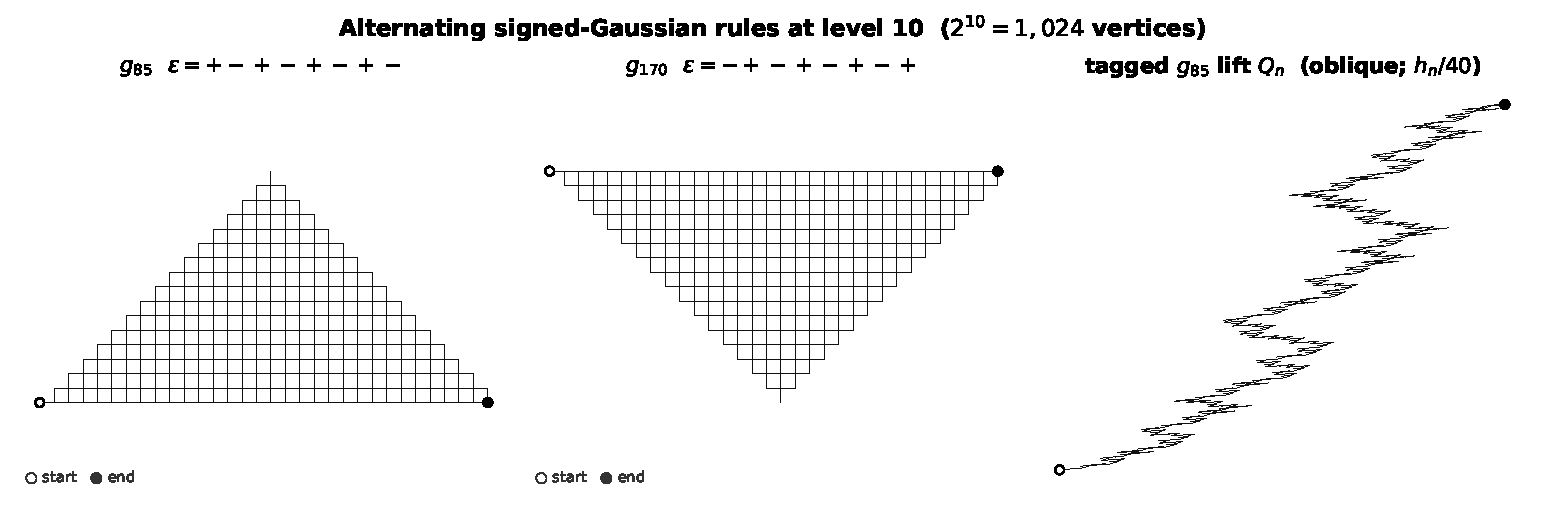
\includegraphics[width=\textwidth]{unit_step_g85_g170_context.pdf}
\vspace{-5pt}
\caption*{Level-10 approximations (1,024 vertices) of the two planar source walks and an oblique view of the tagged $g_{85}$ lift. Open and filled circles mark the initial and final vertices. Height is compressed only for display. These finite pictures provide context; the infinite theorem follows from (1)--(3).}
\end{figure}

The six-dimensional walk itself is the cumulative count of the six vector types, so it has no faithful two-dimensional picture.  The right panel shows its linear shadow $T(P_n)=Q_n$: every unit move in one of six coordinate directions maps to the corresponding spatial vector.  Thus the planar fractal controls which transitions occur, the tagged lift certifies no collinear triple, and the basis encoding enforces unit steps.

\vspace{3pt}
{\footnotesize\textbf{References.}
\begin{enumerate}\setlength{\itemsep}{0pt}\setlength{\parsep}{0pt}\setlength{\topsep}{1pt}
\item[\textup{[1]}] S.~Cambie and E.~Kalviainen, \emph{An infinite small-step $\Z^3$-walk with no collinear triple}, arXiv:2609.01766, 2026.
\item[\textup{[2]}] S.~Cambie, \emph{A unit-step walk in fourteen dimensions}, manuscript, September 5, 2026.
\item[\textup{[3]}] J.~Shallit, \emph{An infinite walk in $\N^{16}$, using only unit steps, with no three collinear points}, manuscript, September 4, 2026.
\end{enumerate}}
\end{document}
